\chapter{Parallelization of the population-based algorithm}
\chaptermark{Parallelization of the population...}
\thispagestyle{empty}

The 
theoretical properties which can be used to approximate the
theoretical speed\-up of parallel population-based algorithms, as evolutionary algorithms (including genetic algorithms), memetic algorithms, particle swarm
optimization, harmony search, etc. are presented in this chapter. The most
frequently method of parallelization employed to population-based algorithm
implements a master-slave model which includes distributing the most
computationally exhausting elements of the algorithm (usually
evaluation of the fitness function, i.e. cost function
calculation) among a number of processors (slaves). The above mentioned master-slave parallelization is seen as easy in programming, therefore the process is popular with practitioners. What is more, if the
master processor keeps the population (and slave processors are
implemented only as computational units for individuals fitness function
evaluation), the solution space is explored in exactly the same
manner as the sequential population-based algorithm. Thus, it is possible to state that we analyze the single-walk parallel population-based algorithm.


\section{Introduction}

Population-based algorithms (genetic, memetic, particle swarm
optimization, etc.) can be characterized by the fact that they
naturally partition onto separate groups of solutions, which are
concurrently processed, that is why they are well-suited to parallelization. 
The usage of population of
individuals allows us to \emph{diversify} the process of searching onto
the whole solution space. However, looking at the process from other perspective, while using cooperation, it
is easy to \emph{intensify} the search after finding a good region
by focusing individuals onto it. Due to its concurrent manner of acting,
population-based algorithms are very handy to parallelize,
particularly in the independent way using multi-start model. Low
level parallelization is not so easy because it usually requires the implementation of the special properties of
the considered problem.

\section{Population-Based Algorithm}\index{Population-Based Algorithm, PBA}

In the population-Based Algorithm (PBA) method\index{method!population-based algorithm} as an iterative technique a population of individuals is implemented to find a global optimum. Each individual of the population
encodes the complete solution, whereas starting population is usually
generated randomly. For instance a genetic algorithm (GA) applies a recombination operator
(crossover) on two solutions in order to introduce diversity of
population. What is more, a mutation operator 
modifying an individual randomly is applied as the insurance against
stagnation of the search process. Even though GAs were
originally associated with the binary representation of a solution, in jobs scheduling area a permutational solution representation is
more popular and useful.

When run concurrently the performance of population-based algorithms, such as GAs, is specially improved. With respect to this two strategies of
parallelization are commonly used:
\begin{enumerate}
\item computations parallelization, in which operations allied to
each individuals (i.e. goal function or genetic operators) are
performed in parallel, as well~as

\item population parallelization in which the population is
partitioned into different parts which can be evolved concurrently
or exchanged.
\end{enumerate}
There are different kinds of parallelization methods
usually applied to population-based algorithms:
\begin{itemize}
\item \emph{Global parallelization.} The model based on the
master-slave type concurrent processes uses the calculations of the
objective function distributed among several slave processors
while the main loop of the population-based algorithm is executed by the
master processor.

\item \emph{Independent runs.} In this approach the parallel method\index{method!parallel} is more efficient through running several versions
of the same algorithm with different parameters on various
processors. The independent runs model can be also
considered as the distribution model without migration.


\item \emph{Distributed (island) model.} This model is historically connected with parallel genetic algorithm and assumes that a
population is partitioned into smaller subpopulations (islands),
for which there are sequential or parallel GAs (usually with different
crossover and mutation parameters) executed. The distinguishing
characteristic of this model is that individuals within a
particular island can occasionally migrate to another island.

\item \emph{Cellular (diffusion) model.} In this model, also historically designed for GA, the
population is mapped onto neighborhood structure, whereas individuals
may only interact with their neighbors. The neighborhood topology
is usually taken from the physical processors connection network,
thus this is a fine-grained parallelism where processors hold just a
few individuals.
\end{itemize}

\noindent The most common
parallelization of parallel population-based algorithms is the distribution model as it can be implemented in
distributed-memory MIMD machines, such as clusters and grids. This
approach leads to coarse-grain parallelization
\cite{boz_2006_4}. Fine-grained parallel implementations of the
cellular (also called diffusion) model are strongly associated to
the machines on which they are executed \cite{alba95}.
Master-slave implementations are available, also as general
frameworks (i.e. ParadisEO of Cahon et al. \cite{alba17}).

There are two approaches presented in this chapter. The first one, in the
Section~\ref{section_sequential}, comes from Cant\'{u}-Paz
\cite{cantu_paz} and we discuss it briefly. The second one,
described in the Section~\ref{section_tree_based}, constitutes a
new idea of the broadcasting time approximation for the
master-slave parallel population-based algorithm.


\section{Sequential broadcasting}\label{section_sequential}


There are two major modules constituting a parallel population-based algorithm based on the master-slave model, namely: (1) communication module, performed
mainly by the master processor which broadcasts a part of
population among slave processors, and (2) computations modules,
executed both on master and slaves, in which evaluation of the
fitness function is done. Here, a notation, taken from
Cant\'{u}-Paz \cite{cantu_paz} is implemented. Let $T_c$ be a time used to send a
portion of data between two processors, whereas $T_f$ denote the
time required to evaluate one individual. Each of processors, i.e.
both master and slaves, evaluates a fraction of the population in
the time $\frac{n T_f}{p}$, where $p$ is the number of processors
and $n$ is the size of the population. Next, it is assumed in this
section that the master broadcasts the data to slaves processors
sequentially, as shown in Figure~\ref{fig_gantt_seq_comm}. The time consumed by population-based operators is omitted as well as by the mutation
(it is usually much shorter than the time of the fitness function
evaluation). It is also assumed that the part of data assigned to each
processor (i.e. the number of individuals evaluated) is the same
both for each slave processor, and for the master processor.
%
\begin{figure}[h]
\centerline{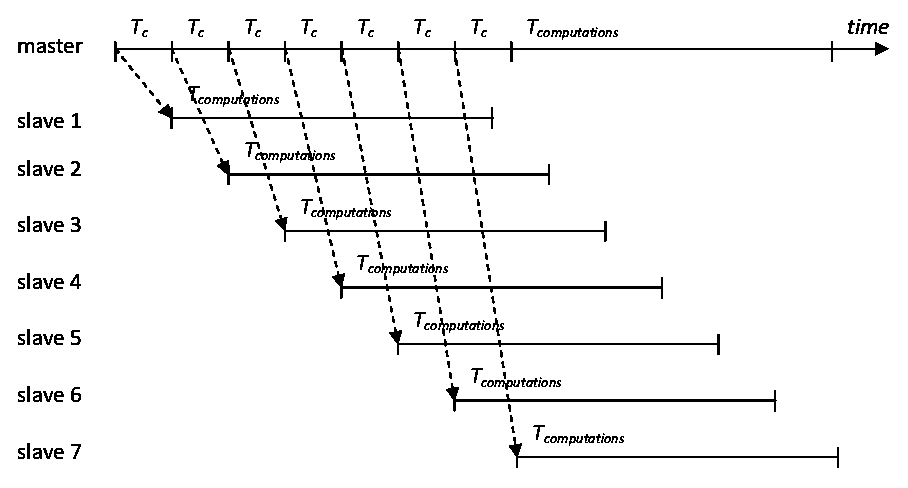
\includegraphics[width=\textwidth]{fig/fig_gantt_seq_comm.eps}}
\caption{Sequential broadcasting in the master-slave parallel
population-based algorithm.} \label{fig_gantt_seq_comm}
\end{figure}


For a sequential model of broadcasting, the parallel running time
is given by the equation
%
\begin{equation}
T_p = p T_c + \frac{n T_f}{p}.
\end{equation}
%
Let us check for which $p$ the $T_p$ is minimal. We denote this
$p$ by $p^*_1$. By calculating $\frac{\partial T_p}{\partial p} = 0$
we obtain
%
\begin{equation}
T_c - \frac{n T_f}{p^2} = 0,
\end{equation}
%
\begin{equation}
p = p^*_1 = \sqrt{\frac{n T_f}{T_c}},
\end{equation}
%
which gives us an optimal number of processors $p^*_1$
minimizing the value of the parallel running time $T_p$.
Calculating the maximum value of the theoretical speedup $S_p$ we
get 
%
\begin{equation}
S_p = \frac{T_s}{T_p} = \frac{n T_f}{p T_c + \frac{n T_f}{p}}.
\end{equation}
%
Substituting the optimal number of processors $p^*_1$ we have
%
$$
S_{p^*_1} = \frac{n T_f}{p^*_1 T_c + \frac{n T_f}{p^*_1}} =
\frac{n T_f}{\sqrt{\frac{n T_f}{T_c}} T_c + \frac{n
T_f}{\sqrt{\frac{n T_f}{T_c}}}}=
$$
%
\begin{equation}
= \frac{n T_f}{\sqrt{n T_f T_c} + \sqrt{\frac{(n T_f)^2}{\frac{n
T_f}{T_c}}}}=\frac{\sqrt{(n T_f)^2}}{2 \sqrt{n T_f
T_c}}=\frac{1}{2} \sqrt{\frac{n T_f}{T_c}} = \frac{1}{2} p^*_1,
\end{equation}
%
which, in case of this model, provides us with a maximal possible speedup of the
single-walk master-slave parallel population-based algorithm.	

Figure~\ref{fig_seq_comm} depicts possible theoretical speedups for
a given ratio $g=\frac{T_f}{T_c}$. The speedup is plotted for
$g=1,2,4$ showing that, with $g$
parameter, linearity of the speedup increases. In practice, $T_f$ is much greater than $T_c$. In such
a situation the parallel algorithm can achieve near-linear speedup
for the number of processors from the range $[1,p^*_1]$. In case of the
number of processors greater than $p^*_1$ speedup quickly
decreases.
%
\begin{figure}[h]
\centerline{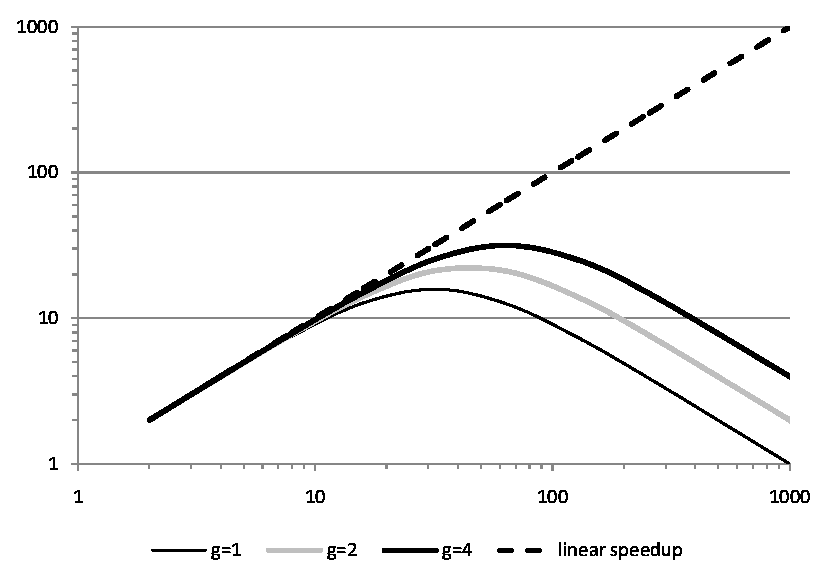
\includegraphics[width=\textwidth]{fig/fig_seq_comm.eps}}
\caption{Theoretical speedups for the \emph{sequential
broadcasting} in the master-slave parallel population-based algorithm.}
\label{fig_seq_comm}
\end{figure}

\section{Tree-based broadcasting}\label{section_tree_based}

Here, a faster model of communication for the master-slave
parallel population-based algorithm is proposed. 
The tree communication scheme is implemented in the broadcasting process, which makes it possible to obtain
logarithmic complexity of the broadcasting process. This
broadcasting scheme needs cooperation of all processors during the
communication process. A scheme of the master-slave parallel
population-based algorithm based on this communication model is shown in
the Figure~\ref{fig_gantt_tree_comm}.
%
\begin{figure}[h]
\centerline{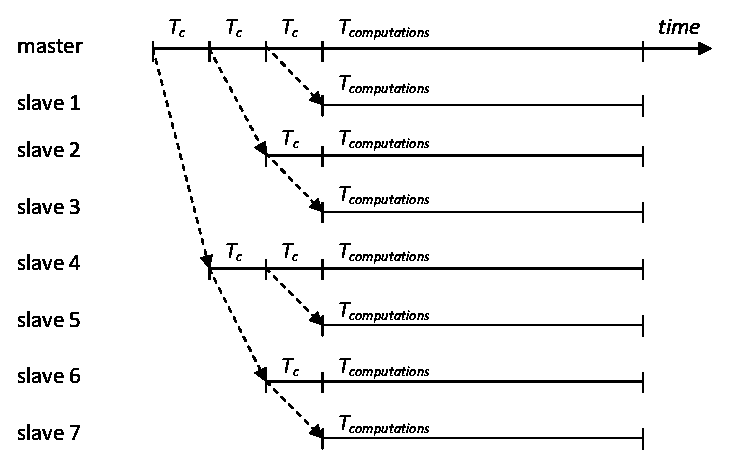
\includegraphics[width=\textwidth]{fig/fig_gantt_tree_comm.eps}}
\caption{Tree-based broadcasting in the master-slave parallel
population-based algorithm.} \label{fig_gantt_tree_comm}
\end{figure}
%


The parallel running time for the tree-based communication model 
$T_p$ is estimated by
%
\begin{equation}
T_p =  T_c \log p + \frac{n T_f}{p}.
\end{equation}
%
When more processors are used, the parallel computations
time $(\frac{n T_f}{p})$ decreases, while the time of
communication $(T_c \log p)$ increases. Such a
processors number $p$ (let us call it $p^*_2$) is required for which $T_p$ is
minimal. By calculating $\frac{\partial T_p}{\partial p} = 0$ it is possible to obtain
%
\begin{equation}
\frac{T_c}{p} - \frac{n T_f}{p^2} = 0
\end{equation}
%
and then
%
\begin{equation}
p = p^*_2 = \frac{n T_f}{T_c},
\end{equation}
%
which provides us with an optimal number of processors $p^*_2$
minimizing the value of the parallel running time $T_p$ for
this model of broadcasting. By calculating the maximum value of the
theoretical speedup $S_p$ the following equation is obtained
%
\begin{equation}
S_p = \frac{T_s}{T_p} = \frac{n T_f}{T_c \log p + \frac{n
T_f}{p}}.
\end{equation}
%
By substituting the optimal number of processors $p^*_2$ we get
%
$$
S_{p^*_2} = \frac{n T_f}{T_c \log p^*_2 + \frac{n T_f}{p^*_2}} =
\frac{n T_f}{\sqrt{T_c \log \frac{n T_f}{T_c}} + \frac{n
T_f}{\frac{n T_f}{T_c}}}=
$$
%
\begin{equation}
= \frac{n T_f}{T_c ( 1+ \log \frac{n T_f}{T_c})} =
\frac{p^*_2}{1+\log p^*_2}.
\end{equation}
%
This equation provides us with a maximal possible speedup for the
tree-base model of broadcasting for the single-walk master-slave
parallel population-based algorithm.

The Figure~\ref{fig_tree_comm} depicts possible theoretical speedups
for a given ratio $g=\frac{T_f}{T_c}$, $g=1,2,4$. As for
sequential communication plotted on the Figure~\ref{fig_seq_comm},
linearity of the speedup increases together with the increase of the $g$
parameter. The parallel algorithm achieves the near-linear speedup
for the number of processors from the range $[1,p^*_2]$. In case when the
number of processors is greater than $p^*_2$ speedup keeps on
increasing.
%
\begin{figure}
\centerline{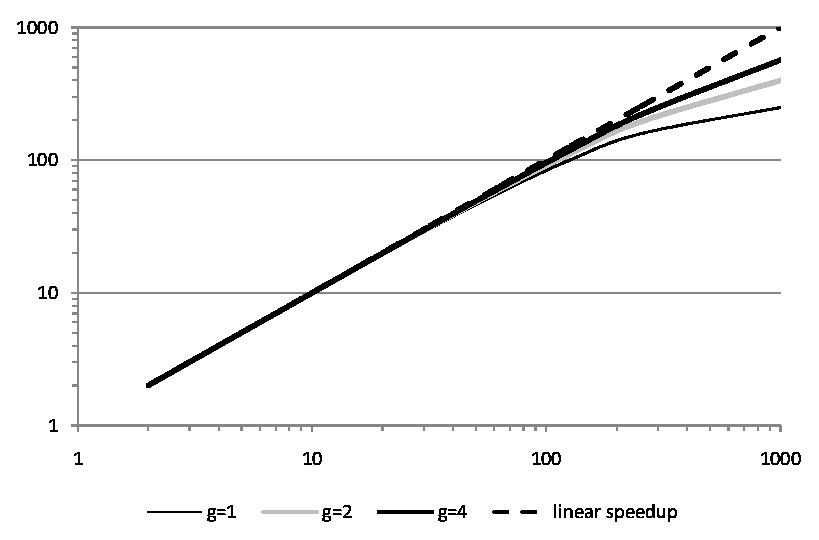
\includegraphics[width=\textwidth]{fig/fig_tree_comm.eps}}
\caption{Theoretical speedups for the \emph{tree-based
broadcasting} in the master-slave parallel population-based algorithm.}
\label{fig_tree_comm}
\end{figure}

\section{Remarks and conclusions}

There were already some theoretical properties of a
single-walk metaheuristics parallelization discussed here which can be used in solving scheduling optimization
problems. The tree-based broadcasting model seems to be more
efficient than the sequential broadcasting model from the
theoretical point of view. In practice, it is possible to 
improve additionally the algorithm’s efficiency by fulfilling
of some processors idle time during the communication phase -- if
this process is executed in the cycle, one generation of the
parallel population-based algorithm after another, the
synchronicity constraint can be eliminated. In such a case the master processor can
execute a communication phase during a communication phase of the
previous generation.


The proposed speedup estimation considered the parallel genetic
algorithm based on the master-slave model of parallelism. The
analyzed approaches provide us with a theoretical approximation of the
optimal number of processors necessary to obtain the highest
speedup. Furthermore, for the master-slave model of
the parallel population-based algorithm with a single population kept by
the master processor it is possible to determine theoretical
upper bounds for obtained speedups.

\begin{thebibliography}{20}

%\bibitem{boz_2010}
%Bo\.{z}ejko W., Uchro\'{n}ski M., Wodecki M. (2010). Parallel hybrid metaheuristics for the  flexible %job shop problem.
%Computers \& Industrial Engineering 59, 323–-333.

%\bibitem{boz_2008_4}
%Bo\.{z}ejko W., Pempera J., Smutnicki C. (2008). Parallel single-thread strategies in scheduling. In: %Artificial Intelligence and Soft
%Computing, Lecture Notes in Artificial Intelligence Vol. 5097, Springer, 995--1006.

%\bibitem{boz_2008_2}
%Bo\.{z}ejko W., Pempera J., Smutnicki C. (2008). Multi-thread parallel metaheuristics for the flow shop %problem. In:
%L. Rutkowski, R. Tadeusiewicz, L.A. Zadeh, J.M. Zurada (Eds.) Artificial Intelligence and Soft Computing, 
%IEEE Computational Intelligence Society - Poland Chapter and the Polish Neural Network Society, 454--462.

\bibitem{boz_2006_4}
Bo\.{z}ejko, W. and Wodecki, M. (2006).
A new inter-island genetic operator for optimization problems with
block properties.   Lecture Notes in Artificial Intelligence Vol. 4029, Springer, 324--333. 

\bibitem{alba17}
Cahon, S., Melab, N., and Talbi, E.-G. (2004).
Paradiseo on condor-mw for optimization on computational grids.
{http://www.lifl.fr/\linebreak {\textasciitilde{}}cahon/cmw/index.html}.

\bibitem{cantu_paz}
Cant\'{u}-Paz, E. (2005).
Theory of parallel genetic algorithms.
In: Alba, E. (Ed.) Parallel Metaheuristics, Wiley, 425--444.
 
\bibitem{Czech}
Czech, Z. (2002).
Three parallel algorithms for simulated annealing.
Lecture Notes in Artificial Intelligence Vol. 2328, Springer, 210--217. 

\bibitem{alba95}
Davidor, Y. (1991).
A naturally occuring niche and species phenomenon: The model and first results.
In:  Proceedings of the Fourth International Conference of Genetic
Algorithms, 257--263.
  
\end{thebibliography}
